\documentclass[10pt,journal,compsoc]{IEEEtran}

% *** CITATION PACKAGES ***
\ifCLASSOPTIONcompsoc
  % IEEE Computer Society needs nocompress option
  % requires cite.sty v4.0 or later (November 2003)
  \usepackage[nocompress]{cite}
\else
  % normal IEEE
  \usepackage{cite}
\fi

\usepackage{lscape}
\usepackage{textcomp}
\usepackage{pgfgantt}
\usepackage{geometry}
\geometry{margin=0.75in}

\begin{document}
\onecolumn

\begin{titlepage}

\begin{flushright}
\textbf{IEEE Std 830-1998} \\
(Revision of \\
IEEE Std 830-1993) \\
\vspace{5mm}
\textbf{IEEE Std 830-1998}
\end{flushright}

\vspace{25mm}

\begin{flushleft}
\begin{bfseries}
	\vskip2mm
	\Huge{Requirements Document for\\ Better Graphics For A Robotics Grasping GUI}\\
	\vspace{30mm}
	\textbf{\huge Shady Robots} \\
	
\end{bfseries}

\vspace{15mm}
\Large{CS461: Senior Software Engineering Project} \\
\Large{Fall 2016} \\

\vspace{10mm}

\today

\end{flushleft}

\newpage

\begin{flushright}
\textbf{IEEE Std 830\texttrademark-1998(R2009)} \\
(Revision of \\
IEEE Std 830-1993) \\
\end{flushright}

\vspace{15mm}

\begin{flushleft}
\begin{bfseries}
	\vskip2mm
	\Huge{Requirements Document for\\ Better Graphics For A Robotics Grasping GUI}\\
	\vspace{30mm}
	\textbf{\huge Shady Robots} \\
	
\end{bfseries}

\vspace{15mm}
\Large{CS461: Senior Software Engineering Project} \\
\Large{Fall 2016} \\

\vspace{10mm}

\today

\vfill

\begin{normalsize}
{\bf Abstract:}
Our customer is using a simulation to create visuals that are used for online data collection.
This simulation is using outdated libraries which result in outdated graphics.
We, as the supplier define the requirements necessary to accomplish our customer's request.
The request being to update the simulation's graphics with warm cool shaders, shadows and silhouettes.

{\bf Keywords:} OpenInventor, OpenGL, OpenRave, shaders, warm cool shaders, silhouettes, shadows, robotic simulation, geometry, visualization, render,
vertex lines, software requirements specification, system requirements specifications
\end{normalsize}
\end{flushleft}

\newpage

\end{titlepage}

\section*{Introduction}
\vspace{3mm}
Currently, our client is using visualizations, of a robot hand grasping objects, to collect data online.
These visualizations are created from a simulation program (OpenRave), the data collected is used to create a model of the human grasp.
However, the current graphics in the simulation are outdated.
It is hard to see and understand the shapes and contact points represented in the scene.
Because of this, users aren't confident in giving proper responses to the simulation.
Thus, the graphics need to be updated to allow meaningful data to be collected. \\


\section*{Participants}
\vspace{3mm}
Cindy Grimm, Matthew Huang, Daniel Goh and Justin Bibler \\ 

\newpage

\tableofcontents

\newpage
\begin{flushleft}
\section{Overview}
\vspace{3mm}
This document describes requirements needed to enhance the current OpenRave simulation. 
Clause 2 lists the references made to other documents. 
Clause 3 provides definitions of specific terms used.
Clause 4 lists the specific requirements that will be met.
This includes the external interface requirements, functional requirements, performance requirements, design constraints, software system attributes, and other requirements.

\section{References}
\vspace{3mm}

Gooch Shading \footnote{\label{note1}ECGLAB. Gooch Shading. Retrieved from: https://lva.cg.tuwien.ac.at/ecg/wiki/doku.php?id=students:gooch}
\vspace{3mm}

IEEE Std 830-1998, IEEE Recommended Practice for Software Requirements Specifications \footnote{\label{note2}IEEE publications are available from the Institute of Electrical and Electronics Engineers, 445 Hoes Lane, P.O. Box 1331, Piscataway, NJ 08855-1331, USA.}
\vspace{3mm}

Shadow Maaping \footnote{\label{note3} Shadow Mapping. LearnOpenGL. Retrieved from: http://learnopengl.com/\#!Advanced-Lighting/Shadows/Shadow-Mapping}
\vspace{3mm}

Silhouette Extraction \footnote{\label{note4}Gooch, Bruce. Silhouette Extraction. Retrieved from: http://www.cs.rutgers.edu/~decarlo/readings/gooch-sg03c.pdf}

\section{Definitions}

\vspace{3mm}
\textbf{Contract:}
A legally binding document agreed upon by the customer and supplier. This includes the technical and organizational requirements, cost, and schedule for a product. A contract may also contain informal but useful information such as the commitments or expectations of the parties involved.

\vspace{3mm}
\textbf{Customer:}
The person, or persons, who pay for the product and usually (but not necessarily) decide the requirements. In the context of this recommended practice the customer and the supplier may be members of the same organization.

\vspace{3mm}
\textbf{Supplier:}
The person, or persons, who produce a product for a customer.

\vspace{3mm}
\textbf{User:}
The person, or persons, who operate or interact directly with the product. The user(s) and the customer(s) are often not the same person(s).

\newpage

\section{Specific requirements}
\vspace{3mm}

\subsection{External interface requirements}
\vspace{3mm}
The purpose of the software's output is to give a visual understanding of the robot's grasping capabilities.
The software will accept an input simulation file (.py file) through the console.
The software will then output a simulation onto a new window.

\subsection{Functional requirements}
\vspace{3mm}
The system shall render the scene and output to a new window.
The rendered scene shall include all 3D objects to be displayed in the scene with correct geometry.
No objects should have clashing vertex lines, and all shapes should be drawn as intended by the user.
Refer to Fig. 1 below.

\begin{figure} [h]
  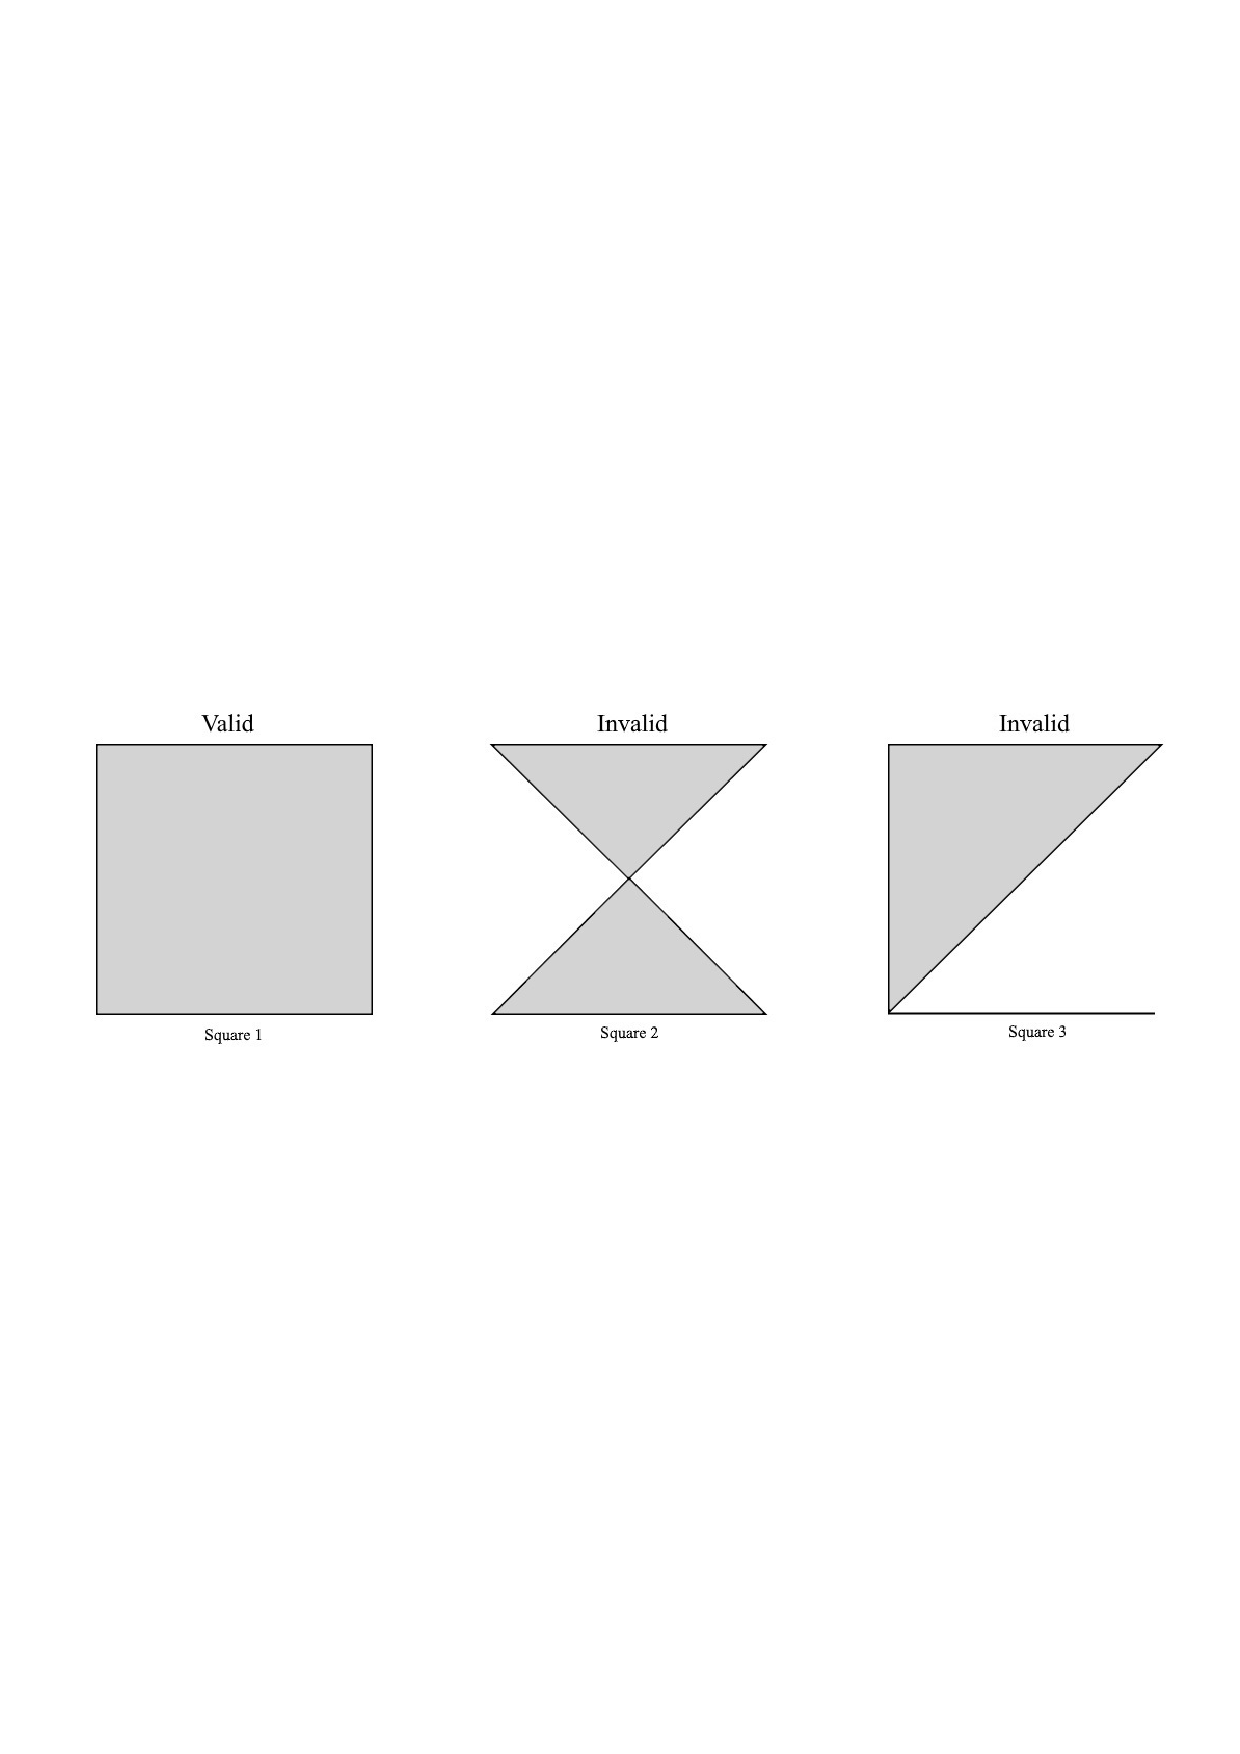
\includegraphics[width=\linewidth]{squares.jpg}
  \caption
{ \newline \hspace{\linewidth}
Square 1: Vertex lines drawn correctly resulting in desired geometry. \newline \hspace{\linewidth}
Square 2: Vertex lines cross resulting in undesired geometry. \newline \hspace{\linewidth}
Square 3: Incorrect vertex line drawing resulting in undesired geometry.}
  \label{fig:squares}
\end{figure}

\vspace{3mm}

The scene shall include:
\subsubsection{Warm cool shaders}
Refer to "Description" section of Gooch Shading listed in this document's references section.

\subsubsection{Shadows}
A dark area or shape produced by a body coming between rays of light and a surface.

\subsubsection{Silhouettes}
Refer to "Definition of a Silhouette" section of Silhouette Extraction listed in this document's references section.

\vspace{3mm}
The system shall continuously re-render the scene until completion of the simulation or software termination.

\subsection{Performance requirements}
\vspace{3mm}
\begin{itemize}
\item The system output should maintain a minimum stable 30FPS on an average modern computer.
\begin{itemize}
\item Modern computer defined by the Oregon State University (OSU) EECS minimum laptop requirements: \\
Intel Core i5 or i7, or AMD A8 and AMD A10 APU
8GB RAM

\end{itemize}
\item The system will only run one simulation per window.
\item The initial scene will be rendered within the first 30 seconds after accepting an input file.
\end{itemize}

\subsection{Design constraints}
\vspace{3mm}
\begin{itemize}
\item The system currently utilizes outdated OpenGL libraries.
\item The location of the main render loop is not known to the customer.
\item OpenRave is not open sourced.
\end{itemize}


\subsection{Software system attributes}
\vspace{3mm}
\subsubsection{Reliability}
\vspace{5mm}
The system shall always run properly created simulations.


\subsubsection{Maintainability}
\vspace{3mm}
The system shall:
\begin{itemize}
\item Be easily maintained and upgraded. 
\item Have well documented and easily testable functions.
\item Have functions with single, clear purposes; they should not overlap in what they do.
\end{itemize}

\subsubsection{Portability}
\vspace{3mm}
The system shall work on Linux operating systems.

\subsection{Other requirements}
\vspace{3mm}
The outdated OpenGL libraries will be updated to utilize OpenGL 3.0 libraries.

\vfill

\newpage

\begin{landscape}
\section{Gantt Chart}
\vfill
\begin{ganttchart}{27}
\gantttitle{2016}{9} 
\gantttitle{2017}{18} \\
\gantttitlelist{10,...,12}{3} 
\gantttitlelist{1,...,6}{3} \\
\ganttgroup{Shady Robots}{1}{27} \\
\ganttbar{Explore and familiarize knowledge with the simulation}{1}{6} \\ % end of november
\ganttlinkedbar{Implement warm cool shaders in simulation}{7}{12} \\ % 2 month
\ganttmilestone{Warm Cool Shaders Implementation Milestone}{12} \\
\ganttlinkedbar{Implement silhouettes in simulation}{13}{15} \\ % 1 month
\ganttmilestone{Silhouettes Implementation Milestone}{15} \\
\ganttbar{Identify render loop}{16}{18} \\ % 3 months
\ganttbar{Switch to 2-pass rendering}{19}{21} \\ % 3 months
\ganttbar{Implement shadows in simulation}{22}{24} \\ % 3 months
\ganttmilestone{Shadows Implementation Milestone}{24} \\
\ganttbar{Aesthetic evaluation}{25}{27} \\
\ganttbar{Finalize and prepare for expo}{25}{27} \\
\ganttlink{elem2}{elem3}
\ganttlink{elem3}{elem4}
\ganttlink{elem4}{elem5}
\ganttlink{elem5}{elem6}
\ganttlink{elem6}{elem7}
\ganttlink{elem7}{elem8}
\ganttlink{elem8}{elem9}
\ganttlink{elem9}{elem10}
\end{ganttchart}
\newline
\begin{center}
Gantt Chart for Shady Robots' Senior Design Project
\end{center}
\vfill
\end{landscape}

\newpage

\null
\vfill

\noindent\begin{tabular}{ll}
\makebox[2.5in]{\hrulefill} & \makebox[2.5in]{\hrulefill}\\
Cindy Grimm & Date\\[4ex]% adds space between the signatures
\makebox[2.5in]{\hrulefill} & \makebox[2.5in]{\hrulefill}\\
Justin Bibler & Date\\[4ex]% adds space between the signatures
\makebox[2.5in]{\hrulefill} & \makebox[2.5in]{\hrulefill}\\
Matthew Huang & Date\\[4ex]% adds space between the signatures
\makebox[2.5in]{\hrulefill} & \makebox[2.5in]{\hrulefill}\\
Daniel Goh & Date\\
\end{tabular}

\end{flushleft}

\end{document}



